\documentclass{article}
\usepackage{graphicx, tikz-cd, float, titlepic, booktabs} % Required for inserting images
\usepackage{pgfplots}
\pgfplotsset{compat=1.15}
\usepackage{mathrsfs}
\usetikzlibrary{arrows}
\usepackage{amsmath, amssymb, amsthm, amsfonts, siunitx, physics, gensymb}
\AtBeginDocument{\RenewCommandCopy\qty\SI}
\usepackage[version=4]{mhchem}
\usepackage[most,many,breakable]{tcolorbox}
\usepackage{xcolor, fancyhdr, varwidth}
\usepackage[Glenn]{fncychap}
%Options: Sonny, Lenny, Glenn, Conny, Rejne, Bjarne, Bjornstrup
\usepackage{hyperref, cleveref}
\usepackage{icomma, enumitem} %comma as decimal and continue enumerate with [resume]
\usepackage{plimsoll} %use standard state symbol with \stst
\usepackage[danish]{babel}
%%%%%%%%%%%%%%%%%%%%%%%%%%%%%%
% SELF MADE COLORS
%%%%%%%%%%%%%%%%%%%%%%%%%%%%%%
\definecolor{myg}{RGB}{56, 140, 70}
\definecolor{myb}{RGB}{45, 111, 177}
\definecolor{myr}{RGB}{199, 68, 64}
\definecolor{mytheorembg}{HTML}{F2F2F9}
\definecolor{mytheoremfr}{HTML}{00007B}
\definecolor{mylenmabg}{HTML}{FFFAF8}
\definecolor{mylenmafr}{HTML}{983b0f}
\definecolor{mypropbg}{HTML}{f2fbfc}
\definecolor{mypropfr}{HTML}{191971}
\definecolor{myexamplebg}{HTML}{F2FBF8}
\definecolor{myexamplefr}{HTML}{88D6D1}
\definecolor{myexampleti}{HTML}{2A7F7F}
\definecolor{mydefinitbg}{HTML}{E5E5FF}
\definecolor{mydefinitfr}{HTML}{3F3FA3}
\definecolor{notesgreen}{RGB}{0,162,0}
\definecolor{myp}{RGB}{197, 92, 212}
\definecolor{mygr}{HTML}{2C3338}
\definecolor{myred}{RGB}{127,0,0}
\definecolor{myyellow}{RGB}{169,121,69}
\definecolor{myexercisebg}{HTML}{F2FBF8}
\definecolor{myexercisefg}{HTML}{88D6D1}
%%%%%%%%%%%%%%%%%%%%%%%%%%%%%%%%%%%%%%%%%%%%%%%%%%%%%%%%%%%%%%%%%%%%%%
% Box environments for theorems and problems
%%%%%%%%%%%%%%%%%%%%%%%%%%%%%%%%%%%%%%%%%%%%%%%%%%%%%%%%%%%%%%%%%%%%%
\setlength{\parindent}{1cm}
%================================
% Question BOX
%================================
\makeatletter
\newtcbtheorem{question}{Opgave}{enhanced,
	breakable,
	colback=white,
	colframe=myb!80!black,
	attach boxed title to top left={yshift*=-\tcboxedtitleheight},
	fonttitle=\bfseries,
	title={#2},
	boxed title size=title,
	boxed title style={%
			sharp corners,
			rounded corners=northwest,
			colback=tcbcolframe,
			boxrule=0pt,
		},
	underlay boxed title={%
			\path[fill=tcbcolframe] (title.south west)--(title.south east)
			to[out=0, in=180] ([xshift=5mm]title.east)--
			(title.center-|frame.east)
			[rounded corners=\kvtcb@arc] |-
			(frame.north) -| cycle;
		},
	#1
}{def}
\makeatother
%================================
% DEFINITION BOX
%================================

\newtcbtheorem[]{Definition}{Definition}{enhanced,
	before skip=2mm,after skip=2mm, colback=red!5,colframe=red!80!black,boxrule=0.5mm,
	attach boxed title to top left={xshift=1cm,yshift*=1mm-\tcboxedtitleheight}, varwidth boxed title*=-3cm,
	boxed title style={frame code={
					\path[fill=tcbcolback]
					([yshift=-1mm,xshift=-1mm]frame.north west)
					arc[start angle=0,end angle=180,radius=1mm]
					([yshift=-1mm,xshift=1mm]frame.north east)
					arc[start angle=180,end angle=0,radius=1mm];
					\path[left color=tcbcolback!60!black,right color=tcbcolback!60!black,
						middle color=tcbcolback!80!black]
					([xshift=-2mm]frame.north west) -- ([xshift=2mm]frame.north east)
					[rounded corners=1mm]-- ([xshift=1mm,yshift=-1mm]frame.north east)
					-- (frame.south east) -- (frame.south west)
					-- ([xshift=-1mm,yshift=-1mm]frame.north west)
					[sharp corners]-- cycle;
				},interior engine=empty,
		},
	fonttitle=\bfseries,
	title={#2},#1}{def}
\newtcbtheorem[]{definition}{Definition}{enhanced,
	before skip=2mm,after skip=2mm, colback=red!5,colframe=red!80!black,boxrule=0.5mm,
	attach boxed title to top left={xshift=1cm,yshift*=1mm-\tcboxedtitleheight}, varwidth boxed title*=-3cm,
	boxed title style={frame code={
					\path[fill=tcbcolback]
					([yshift=-1mm,xshift=-1mm]frame.north west)
					arc[start angle=0,end angle=180,radius=1mm]
					([yshift=-1mm,xshift=1mm]frame.north east)
					arc[start angle=180,end angle=0,radius=1mm];
					\path[left color=tcbcolback!60!black,right color=tcbcolback!60!black,
						middle color=tcbcolback!80!black]
					([xshift=-2mm]frame.north west) -- ([xshift=2mm]frame.north east)
					[rounded corners=1mm]-- ([xshift=1mm,yshift=-1mm]frame.north east)
					-- (frame.south east) -- (frame.south west)
					-- ([xshift=-1mm,yshift=-1mm]frame.north west)
					[sharp corners]-- cycle;
				},interior engine=empty,
		},
	fonttitle=\bfseries,
	title={#2},#1}{def}

\newtcbtheorem{theo}%
    {Theorem}{}{theorem}
\newtcolorbox{prob}[1]{colback=red!5!white,colframe=red!50!black,fonttitle=\bfseries,title={#1}}
%================================
% NOTE BOX
%================================

\usetikzlibrary{arrows,calc,shadows.blur}
\tcbuselibrary{skins}
\newtcolorbox{note}[1][]{%
	enhanced jigsaw,
	colback=gray!20!white,%
	colframe=gray!80!black,
	size=small,
	boxrule=1pt,
	title=\textbf{Note:},
	halign title=flush center,
	coltitle=black,
	breakable,
	drop shadow=black!50!white,
	attach boxed title to top left={xshift=1cm,yshift=-\tcboxedtitleheight/2,yshifttext=-\tcboxedtitleheight/2},
	minipage boxed title=1.5cm,
	boxed title style={%
			colback=white,
			size=fbox,
			boxrule=1pt,
			boxsep=2pt,
			underlay={%
					\coordinate (dotA) at ($(interior.west) + (-0.5pt,0)$);
					\coordinate (dotB) at ($(interior.east) + (0.5pt,0)$);
					\begin{scope}
						\clip (interior.north west) rectangle ([xshift=3ex]interior.east);
						\filldraw [white, blur shadow={shadow opacity=60, shadow yshift=-.75ex}, rounded corners=2pt] (interior.north west) rectangle (interior.south east);
					\end{scope}
					\begin{scope}[gray!80!black]
						\fill (dotA) circle (2pt);
						\fill (dotB) circle (2pt);
					\end{scope}
				},
		},
	#1,
}
%================================
% EXAMPLE BOX
%================================
\newtcbtheorem[number within=section]{Example}{Example}
{%
	colback = myexamplebg
	,breakable
	,colframe = myexamplefr
	,coltitle = myexampleti
	,boxrule = 1pt
	,sharp corners
	,detach title
	,before upper=\tcbtitle\par\smallskip
	,fonttitle = \bfseries
	,description font = \mdseries
	,separator sign none
	,description delimiters parenthesis
}
{ex}
%================================
% THEOREM BOX
%================================

\tcbuselibrary{theorems,skins,hooks}
\newtcbtheorem[number within=section]{Theorem}{Theorem}
{%
	enhanced,
	breakable,
	colback = mytheorembg,
	frame hidden,
	boxrule = 0sp,
	borderline west = {2pt}{0pt}{mytheoremfr},
	sharp corners,
	detach title,
	before upper = \tcbtitle\par\smallskip,
	coltitle = mytheoremfr,
	fonttitle = \bfseries\sffamily,
	description font = \mdseries,
	separator sign none,
	segmentation style={solid, mytheoremfr},
}
{th}

%%%%%%%%%%%%%%%%%%%%%%%%%%%%%%%%%%%%%%%%%%%%%%%%%%%%%%%%%%%%%%%%%
% SELF MADE COMMANDS
%%%%%%%%%%%%%%%%%%%%%%%%%%%%%%
\newcommand{\sol}{\setlength{\parindent}{0cm}\textbf{\textit{Løsning:}}\setlength{\parindent}{1cm}}
%%%%%%%%%%%%%%%%%%%%%%%%%%%%%%%%%
\usepackage[tmargin=2cm,rmargin=1in,lmargin=1in,margin=0.85in,bmargin=2cm,footskip=.2in]{geometry}\pagestyle{fancy}
\lhead{Minrui Kevin Zhou 3.b}
\rhead{Aflevering 35}

\title{Aflevering 35\\
{\Large \textbf{3.b mat A}}}
\author{Kevin Zhou}
\date{\today}

\begin{document}
\maketitle
\newpage
\begin{question}{}{}
  På figuren ses banekurven for vektorfunktionen $\vec{s}$ givet ved

$$\vec{s}(t)=\begin{pmatrix}-\dfrac{1}{2}t^3+t^2+4t+5\\\\\dfrac{1}{3}t^3-2t^2+3t+4\end{pmatrix}.$$

\begin{itemize}
  \item[a.] Bestem hastighedsvektoren $\vec{v}(t)$.
  \item[b.] Bestem de $t$-værdier, hvor banekurven har en vandret tangent.
\end{itemize}
\end{question}
\sol \\
\textbf{a.}
Hastighedsvektoren er den afledede funktion af vektorfunktionen $\va{s}$.
\begin{equation*}
\begin{split}
  \va{v}(t)&=\va{s}'(t)\\
  &=\mqty(\dv{t} \left(-\dfrac{1}{2}t^3+t^2+4t+5\right) \\ \dv{t} \left(\dfrac{1}{3}t^3-2t^2+3t+4\right) ) \\
  &=\mqty(-\frac{3}{2}t^2+2t+4\\ t^2-4t+3)
\end{split}
\end{equation*}
\textbf{b.}
Da $\va{v}(t)$ altid er tangent til banekurven for $\va{s} (t)$, så må banekurven have en vandret tangent, når $\va{v}(t)$'s komposant i $y$-retningen er 0.
Dette er tilfældet, når
\begin{equation*}
\begin{split}
  t^2-4t+3=0 &\iff (t-1)(t-3)=0\\
  &\iff t=1 \lor t=3
\end{split}
\end{equation*}
Banekurven har altså en vandret tangent når $t=1$ eller $t=3$. 

\begin{question}{}{}
 En funktion $f$ af to variable er givet ved
$$f(x,y)=2x^4\cdot y+7x-y\:.$$
\begin{itemize}
  \item[a.] Bestem $f_x^{\prime}(x,y)$
  \item[b.] Bestem $f_y^{\prime}(x,y)$ 
\end{itemize}
\end{question}
\sol \\
\textbf{a.}
Vi beregner den partielle afledede af $f(x,y)$ mht. $x$. 
\begin{equation*}
\begin{split}
  f_x'(x,y)&=\pdv{x} \left(2x^4 \cdot y + 7x-y\right) \\
  &=8x^3 \cdot y + 7
\end{split}
\end{equation*}
\textbf{b.}
Vi beregner den partielle afledede af $f(x,y)$ mht. $y$. 
\begin{equation*}
\begin{split}
  f_y'(x,y)&=\pdv{y} \left(2x^4 \cdot y + 7x - y\right) \\
  &=2x^4-1
\end{split}
\end{equation*}

\begin{question}{}{}
  Befolkningsudvikilingen i Taiwan i perioden 1996-2019 kan i en model beskrives ved differentialligningen
  \[
\frac{dP}{dt}=0,003641\cdot P\cdot(23,95-P)
  \] 
hvor $P(t)$ er antalle af indbyggere i Taiwan (målt i millioner), og $t$ er antal år efter 1996.
I 1996 var der 21,53 millioner indbyggere i Taiwan.
\begin{itemize}
  \item[a.] Bestem en forskrift for P.
  \item[b.] Bestem $P^{\prime}(23)$, og forklar betydningen af dete tal.
\end{itemize}
\end{question}
\sol \\
\textbf{a.}
Siden der for en ligning af formen
\[
y'=ay(M-y), \quad a>0, M>0
\] 
gælder, at den har de ikke-negative, voksende løsninger 
\[
f(x)= \frac{M}{1+c e^{-aMx} }, \quad c \in \mathbb{R}^+, x \in \mathbb{R}
\] 
så må en forskrift for $P$ være af formen 
\begin{equation*}
\begin{split}
  P(t)&=\frac{23,95}{1+c e^{-0,003641 \cdot 23,95 \cdot t} }\\
  &=\frac{23,95}{1+c e^{-0,08720195\cdot t} }\\
\end{split}
\end{equation*}
og da $P(0)=21,53$, kan vi finde $c$
\begin{equation*}
\begin{split}
  P(0)=21,53 &\iff \frac{23,95}{1+c e^{-0,08720195\cdot 0} } =21,53\\
  &\iff c=\frac{23,95}{21,53}-1\\
  &\iff c=0,112401301
\end{split}
\end{equation*}
Altså er en forskrift for $P$
\[
P(t)=\frac{23,95}{1+0,112401301 e^{-0,08720195t} }
\] 
\textbf{b.}
Vi finder først den afledede funktion af $P$ med kædereglen. 
\begin{equation*}
\begin{split}
  P'(t)&=-\frac{23,95 \cdot \left(-0,009801613 e^{-0,08720195 t} \right) }{\left( 1+0,112401301 e^{-0,08720195t} \right)^2}\\
  &=-\frac{-0,234748622 e^{-0,08720195t } }{\left( 1+0,112401301 e^{-0,08720195t} \right)^2}
\end{split}
\end{equation*}
Vi kan nu bestemme $P'(23)$.
\begin{equation*}
\begin{split}
  P'(23)&=-\frac{-0,234748622 e^{-0,08720195 \cdot 23} }{\left( 1+0,112401301 e^{-0,08720195 \cdot 23} \right)^2}\\
  &\approx -0,0307
\end{split}
\end{equation*}
Det betyder altså, at antallet af indbyggere i Taiwan i år 2019 aftager med $0,0307$ millioner indbyggere per år. 

\begin{question}{}{}
 I 2001 fandt amerikanske og canadiske forskere, at sammenhængen mellem den oplevede temperatur og den aktuelle temperatur ved forskellige vindhastigheder, det såkaldte "windchill indeks", kan beskrives ved
$$f(t,v)=13,3+0,62\cdot t-13,95\cdot v^{0,16}+0,486\cdot t\cdot v^{0,16},$$
  hvor $f(t,v)$ er "windchill indekset" (målt i °C), $t$ er den aktuelle målte temperatur (målt i $\unit{\celsius}$, og $v$ er vindhastigheden (målt i m/s).
  \begin{itemize}
    \item[a.] Bestem $f(-5,20)$, og forklar betydningen af værdien.
    \item[b.] Bestem den vindhastighed, der ved en temperatur på $-3^{\circ}$C giver et "windchill indeks" på $-10 \;\unit{\celsius} $.
  \end{itemize}
\end{question}
\sol \\
\textbf{a.}
Vi bestemmer $f(-5,20)$.
\begin{equation*}
\begin{split}
  f(-5,20)&=13,3 + 0,62 \cdot \left(-5\right) -13,95 \cdot 20 ^{0,16}+0,486 \cdot \left(-5\right) \cdot 20 ^{0,16}\\
  &\approx -16,25
\end{split}
\end{equation*}
Det betyder altså, at når den aktuelle temperatur er $-5 \;\unit{\celsius} $, og vindhastigheden er $20 \;\unit{m/s} $, så er windchill indekset $-16,25 \;\unit{\celsius} $.\\[1ex]
\textbf{b.}
Vi løser da ligningen $f(-3,v)= -10$.
\begin{equation*}
\begin{split}
  f(-3,v)= -10 &\iff 13,3+0,62 \cdot \left(-3\right) - 13,95 \cdot v ^{0,16}+0,486 \cdot \left(-3\right) \cdot v ^{0,16}=-10\\
  &\iff 23,3 -1,86 - \left(13,95+1,458\right) \cdot v ^{0,16}=0\\
  &\iff 15,408 \cdot v ^{0,16}=21,44\\
  &\iff v=\left(\frac{21,44}{15,408}\right)^{\frac{1}{0,16}} \approx 7,884
\end{split}
\end{equation*}
Ved en temperatur på $-3 \;\unit{\celsius} $ skal vindhastigheden altså være $7,884 \;\unit{m/s} $ for at få et windchill indeks på $-10 \;\unit{\celsius} $. 

\begin{question}{}{}
  En funktion $f$ er givet ved 
  $f(x,y)=10-2x^2-y^2$, hvor $2x^2+y^2 \leq 10$.
\begin{itemize}
  \item[a.] Tegn et konturplot med niveaukurver for $f$.
  \item[b.] Tegn grafen for $f$.
\end{itemize}
\end{question}
\sol \\
\textbf{a.}
Et konturplot med niveakurver for $f$ ses i \cref{fig:kontur}.
\begin{figure}[H]
\begin{center}
  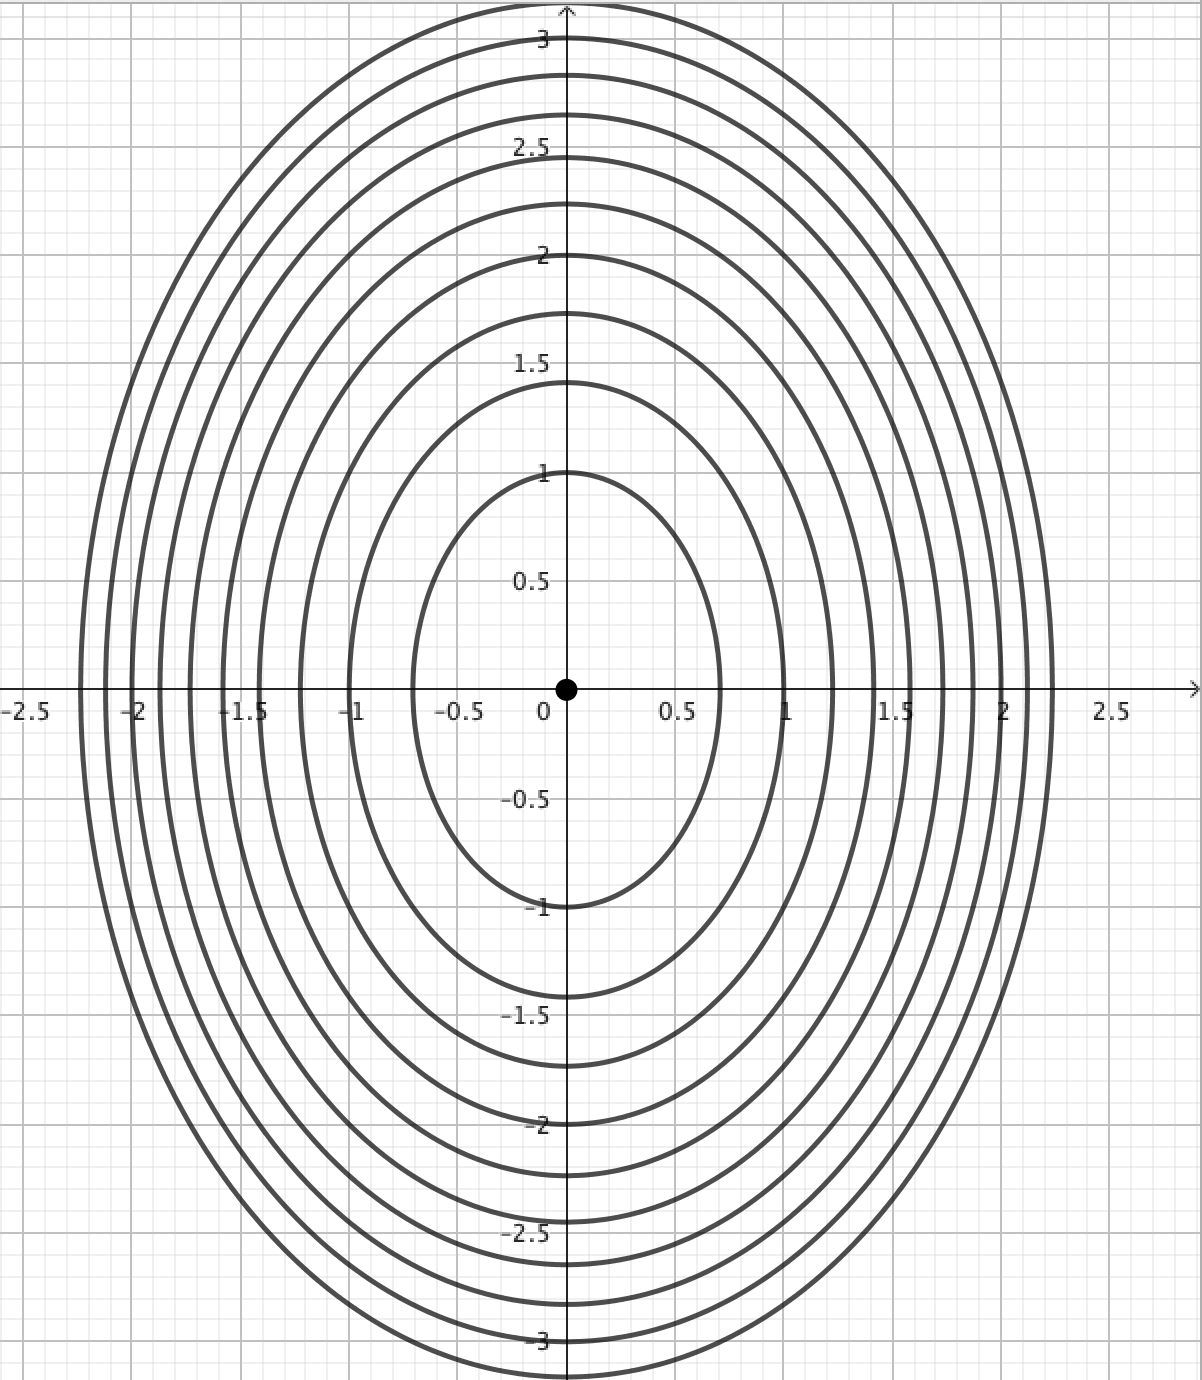
\includegraphics[scale=0.4]{konturplot.png }
\end{center}
\caption{Konturplot for $f$ tegnet i GeoGebra }
\label{fig:kontur}
\end{figure}
\noindent \textbf{b.}
Grafen for ses i \cref{fig:graf}.
\begin{figure}[H]
\begin{center}
  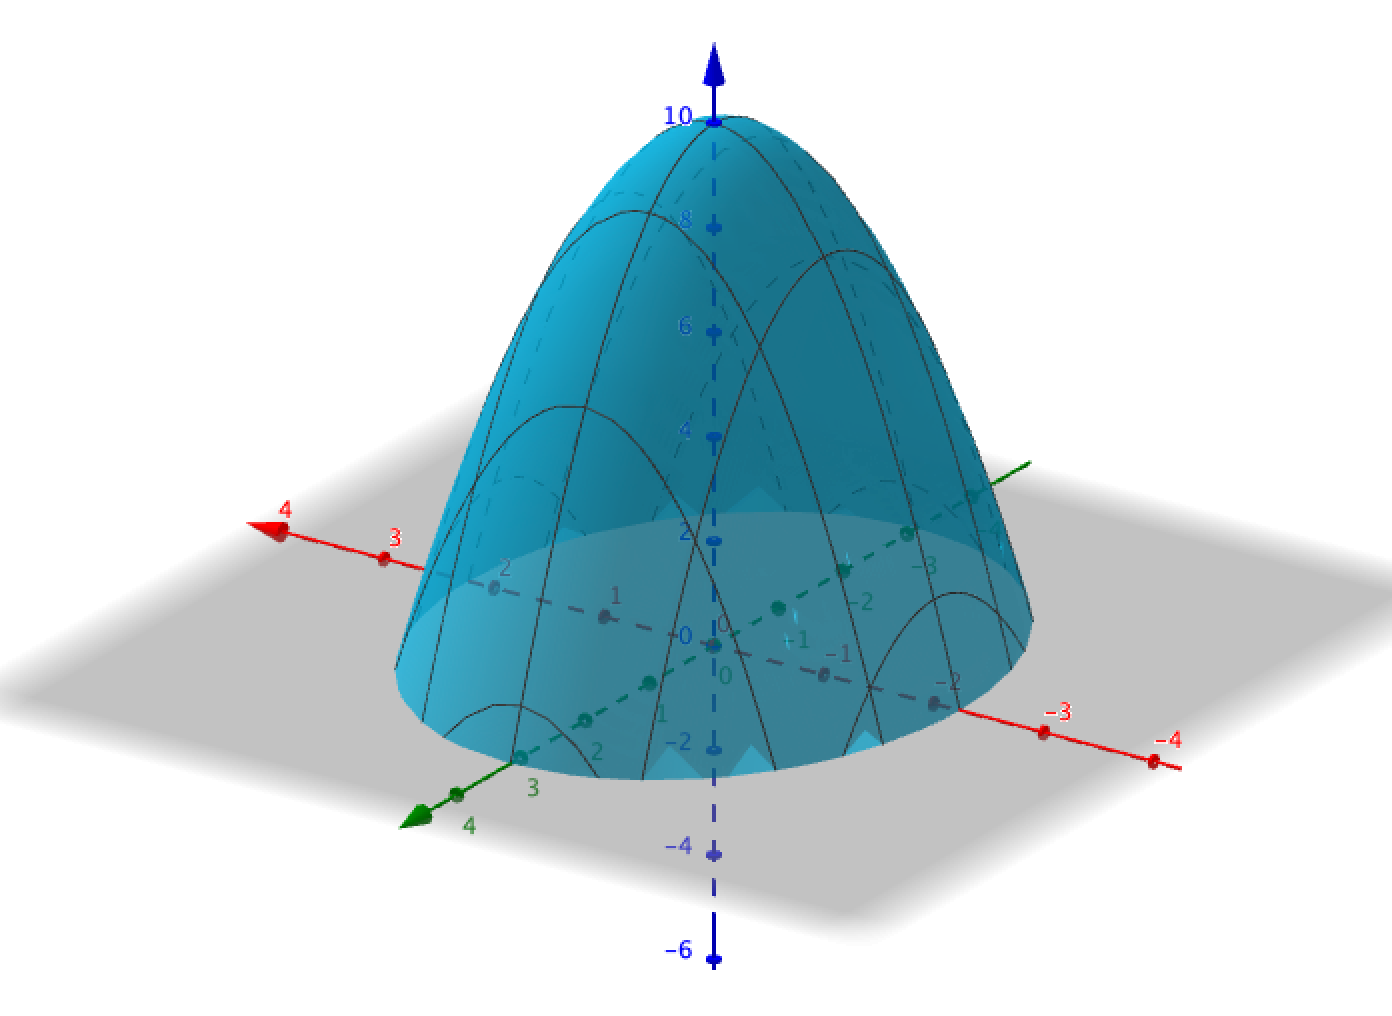
\includegraphics[scale=0.5]{graf.png}
\end{center}
\caption{Grafen for $f$ tegnet i GeoGebra}
\label{fig:graf}
\end{figure}

\end{document}
